% !TeX root = ../Tempel-Daniel.tex
\chapter{Production Architecture for AI Systems}
\label{chap:production}

The previous chapter described how the agent harness coordinates model calls, context construction, tools and task state. Production deployment adds another problem: these operations must remain reliable and responsive under changing workloads while controlling resource use and cost.

Figure~\ref{fig:production-architecture} separates two layers with different workloads. The \textbf{agent execution layer} coordinates retrieval, tools and task state, while the \textbf{model-serving layer} provides inference and manages computational resources. Their workloads differ: an agent task may wait for tests or external operations, whereas model servers process many concurrent inference requests competing for GPU memory and compute.

This chapter therefore focuses on model routing, efficient LLM serving and resilient execution of long-running agent tasks. These mechanisms should be evaluated against task-success, latency, availability and cost objectives rather than throughput or GPU utilisation alone.

\begin{center}
\begin{minipage}{\linewidth}
\centering
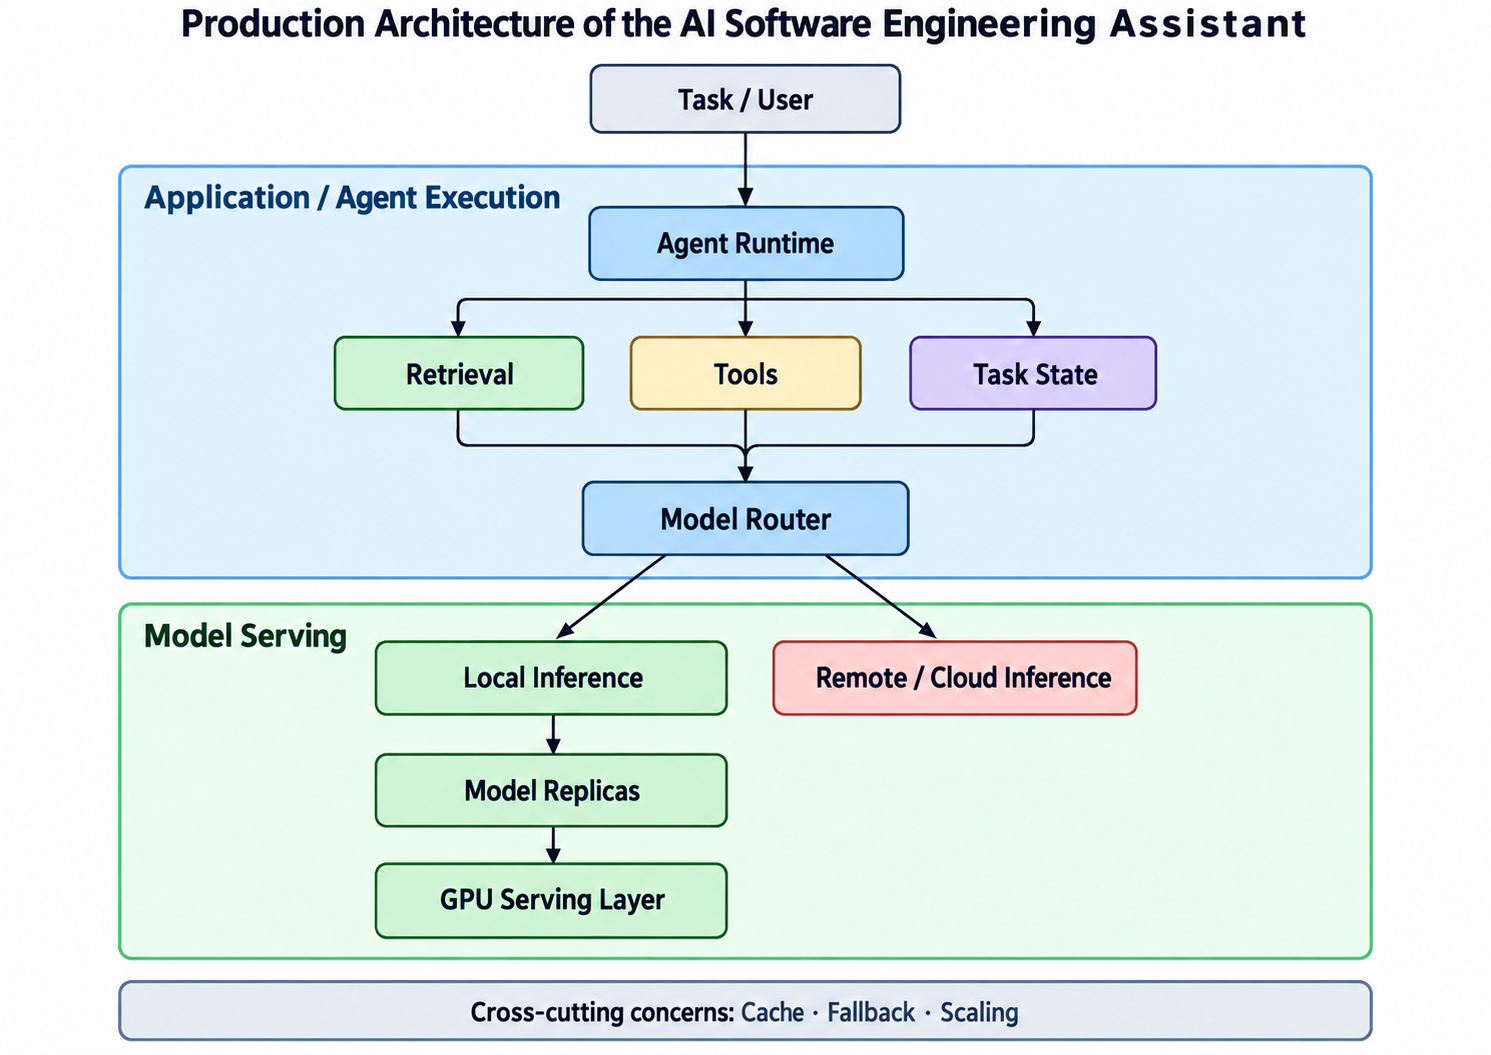
\includegraphics[width=\linewidth]{images/production-architecture.png}
\captionof{figure}{Production architecture of the AI Software Engineering Assistant, separating agent execution from model serving and showing routing between eligible local and remote model deployments.}
\label{fig:production-architecture}
\end{minipage}
\end{center}

\section{Model routing and deployment}

Chapter~\ref{chap:benchmarks} treated model selection as an evaluation problem. In production, several suitable configurations may coexist because individual inference steps have different capability, latency, data-handling and cost requirements.

A \textbf{model router} selects an eligible deployment for a request. Deployments that violate required context length, tool capabilities or data-handling constraints should first be excluded; routing can then optimise among the remaining alternatives for quality, latency, cost or availability.

Static routing can assign known workloads to particular models, such as test-log summarisation to a smaller model and repository modification to a coding-specialised model. Dynamic routing instead considers the current request or task state. RouteLLM demonstrates this general principle by routing between stronger and weaker models to optimise the cost-quality trade-off rather than always invoking the stronger model \parencite{ong2024routellm}.

Routing can also support \textbf{escalation}. For \emph{Fix GitHub issue \#42 and verify the solution}, repeated inability to resolve a verified implementation problem within a configured attempt budget may justify a stronger model. A failed test alone is insufficient evidence, since it may result from the environment, an existing failure or an ordinary intermediate error. When switching models, the current goal, constraints, changes and verification evidence must remain available.

Deployment location provides another routing dimension. Local inference can provide data locality and controlled capacity, while remote inference can provide elastic capacity or capabilities unavailable locally. Hybrid routing can combine both where data-handling policies permit. Operational ownership should be distinguished from location: a self-hosted model may run on rented cloud GPUs, whereas a usage-priced inference API is managed by an external provider.

Finally, \textbf{model routing} chooses a model or deployment, while \textbf{replica routing} chooses a running instance of that deployment. Ray Serve LLM separates these levels and can additionally consider prefix-cache locality when selecting replicas \parencite{ray-routing}.

\section{Latency, cost and efficient LLM serving}

Generative inference contains two different phases. During \textbf{prefill}, the model processes the input tokens; during \textbf{decode}, it generates output autoregressively. \textbf{Time to First Token (TTFT)} measures the elapsed time from request submission to the first output token at a defined measurement boundary. \textbf{Time per Output Token (TPOT)} describes the average time required for subsequent generated tokens. DistServe treats TTFT and TPOT as separate serving objectives because prefill and decode have different computational characteristics \parencite{zhong2024distserve}.

For the assistant, inference latency is only one part of task latency. More uncached input tokens increase prefill work, while longer outputs increase decode work. Issue \#42 may additionally involve several model calls, repository searches, modifications and test runs. End-to-end completion time therefore also includes queueing, tools and retries. Measurements associated with the task identifier can separate these components and reveal the actual bottleneck.

Efficient serving also depends on concurrent execution. Batching improves GPU utilisation by processing several sequences together, but fixed batches are inefficient when autoregressive sequences finish at different times. Orca introduced \textbf{iteration-level scheduling}, allowing the active request set to change between generation iterations \parencite{yu2022orca}. This principle enables continuous batching, where completed sequences can be replaced by new work.

GPU memory creates another constraint. The KV cache grows with active sequences and can limit concurrency even when compute remains available. PagedAttention uses paging-inspired KV-cache management to reduce fragmentation and duplication; the accompanying vLLM system improved serving throughput under the evaluated workloads \parencite{kwon2023pagedattention}.

Prompt caching, introduced in Chapter~\ref{chap:context-memory}, reduces repeated prefill work when requests share a stable prefix. vLLM's Automatic Prefix Caching reuses previously computed KV-cache blocks for matching prefixes. This can reduce computation and TTFT, although retained cache blocks also consume finite serving memory \parencite{vllm-prefix-caching}.

Serving efficiency directly affects cost. Usage-priced inference APIs typically charge according to processed and generated usage, while provisioned self-hosted capacity incurs cost while compute resources remain allocated. Batching, cache reuse and routing can therefore improve effective cost by increasing useful work per unit of compute or avoiding unnecessarily expensive model calls.

However, high utilisation is not itself the objective. Aggressive concurrency may improve throughput while increasing queueing latency. Serving configurations should therefore be compared under defined latency and availability requirements. For the assistant, the \texttt{cost per successful task} metric introduced in Chapter~\ref{chap:benchmarks} remains more useful than the price of an isolated inference request.

\section{Resilient and scalable agent execution}

A software-engineering task may remain active much longer than one inference request while waiting for tests, CI or another external operation. Its lifetime should therefore be independent of both the original HTTP request and a particular worker process.

Figure~\ref{fig:long-running-task-execution} shows queued work advancing through workers while durable task state remains outside them. A persistent task identifier connects resumed execution to the same task.

\begin{center}
\begin{minipage}{\linewidth}
\centering
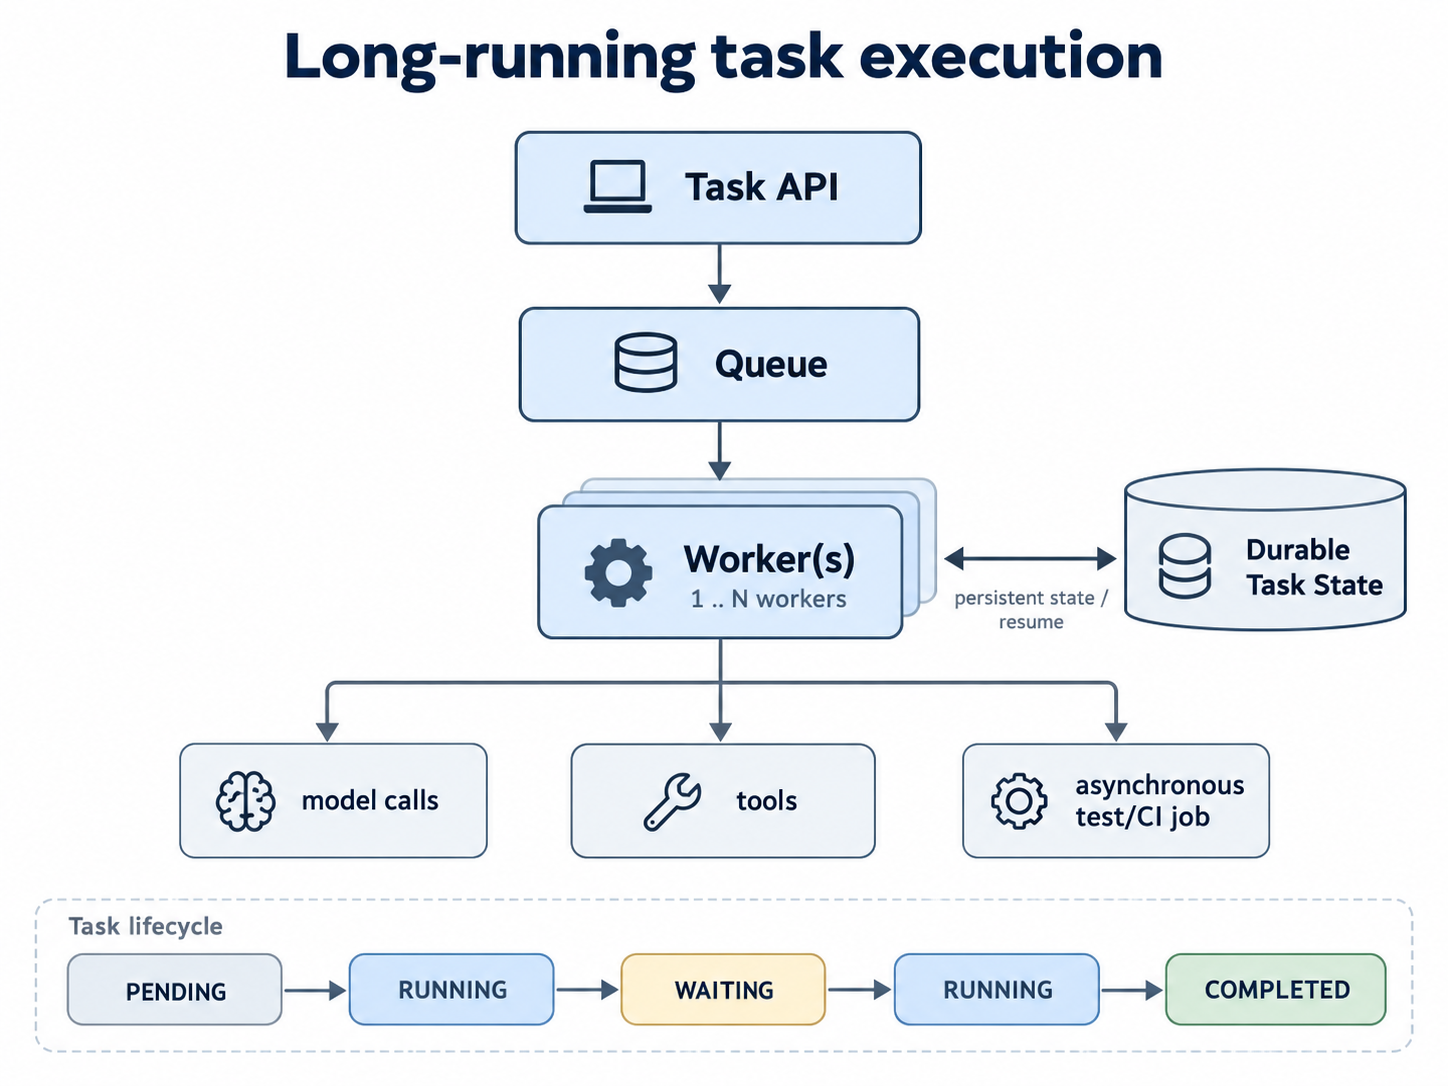
\includegraphics[width=\linewidth]{images/long-running-task-execution.png}
\captionof{figure}{Queue-based execution of a long-running assistant task in which durable orchestration state and recoverable execution artefacts allow processing to resume across asynchronous operations or worker failures.}
\label{fig:long-running-task-execution}
\end{minipage}
\end{center}

The external state store decouples progress from a worker, but a persisted checkpoint alone is insufficient for recovery. If it records that a patch was applied but the modified files existed only on the failed worker's local disk, another worker cannot continue verification. Recovery requires both \textbf{durable orchestration state} and access to the corresponding \textbf{execution artefacts}, such as a persistent workspace or a reproducible combination of repository revision and stored patch. Externally running CI or test jobs also require durable identifiers.

For issue \#42, these references let a replacement worker recover the relevant code and test environment and resume verification.

Recovery also requires task ownership. Queues and persisted state alone do not prevent a stale worker and a replacement worker from concurrently modifying the same task. Task claiming should therefore ensure that only the currently valid execution can commit task progress.

Durable workflow systems provide one implementation approach. Temporal, for example, records workflow Event History and reconstructs workflow state through replay after worker failure \parencite{temporal-workflow}. This restores orchestration progress but does not automatically recover worker-local files or guarantee exactly-once execution of external operations.

The retry distinction established in Section~\ref{sec:agent-task-state} also applies across workers: side effects require outcome reconciliation or an available idempotency mechanism, while infrastructure failures may justify bounded retries, delayed execution or another eligible deployment. Recovery should preserve existing task progress.

Queues also separate incoming demand from execution capacity. If tasks arrive faster than workers can process them, excess work can wait while additional worker or model replicas increase capacity. Horizontal scaling adds replicas, whereas vertical scaling assigns more resources to an existing instance \parencite{kubernetes2026autoscaling}.

Autoscaling should follow the constrained resource: adding workers cannot relieve a saturated model deployment or another limiting dependency. CPU utilisation may be uninformative when workers are waiting for inference; queue depth, ongoing requests or latency can be more useful. Ray Serve can adjust replica counts based on ongoing requests per replica \parencite{ray-autoscaling}.

Replica count and physical compute capacity should also be distinguished. Scaling an application to zero replicas reduces its resource use, but monetary savings depend on whether the underlying GPU capacity can also be released or reused. Keeping ready capacity instead reduces cold-start latency at the cost of idle resources.

Finally, incoming work must remain bounded. If demand continuously exceeds processing capacity, an unbounded queue only turns overload into growing latency and storage consumption. \textbf{Backpressure} limits or delays new work when downstream capacity is exhausted, while priority policies can reserve capacity for interactive tasks over background work.

These mechanisms are deployment choices whose value depends on workload, latency requirements and failure tolerance. As more models, workers and external services participate in execution, controlling their access to repositories and executable capabilities becomes increasingly important. This leads to the next chapter on security and sandboxing for AI agents.
